% Options for packages loaded elsewhere
\PassOptionsToPackage{unicode}{hyperref}
\PassOptionsToPackage{hyphens}{url}
%
\documentclass[
]{article}
\usepackage{lmodern}
\usepackage{amssymb,amsmath}
\usepackage{ifxetex,ifluatex}
\ifnum 0\ifxetex 1\fi\ifluatex 1\fi=0 % if pdftex
  \usepackage[T1]{fontenc}
  \usepackage[utf8]{inputenc}
  \usepackage{textcomp} % provide euro and other symbols
\else % if luatex or xetex
  \usepackage{unicode-math}
  \defaultfontfeatures{Scale=MatchLowercase}
  \defaultfontfeatures[\rmfamily]{Ligatures=TeX,Scale=1}
\fi
% Use upquote if available, for straight quotes in verbatim environments
\IfFileExists{upquote.sty}{\usepackage{upquote}}{}
\IfFileExists{microtype.sty}{% use microtype if available
  \usepackage[]{microtype}
  \UseMicrotypeSet[protrusion]{basicmath} % disable protrusion for tt fonts
}{}
\makeatletter
\@ifundefined{KOMAClassName}{% if non-KOMA class
  \IfFileExists{parskip.sty}{%
    \usepackage{parskip}
  }{% else
    \setlength{\parindent}{0pt}
    \setlength{\parskip}{6pt plus 2pt minus 1pt}}
}{% if KOMA class
  \KOMAoptions{parskip=half}}
\makeatother
\usepackage{xcolor}
\IfFileExists{xurl.sty}{\usepackage{xurl}}{} % add URL line breaks if available
\IfFileExists{bookmark.sty}{\usepackage{bookmark}}{\usepackage{hyperref}}
\hypersetup{
  pdftitle={Statistical Inference Project},
  pdfauthor={JN Gabra},
  hidelinks,
  pdfcreator={LaTeX via pandoc}}
\urlstyle{same} % disable monospaced font for URLs
\usepackage[margin=1in]{geometry}
\usepackage{color}
\usepackage{fancyvrb}
\newcommand{\VerbBar}{|}
\newcommand{\VERB}{\Verb[commandchars=\\\{\}]}
\DefineVerbatimEnvironment{Highlighting}{Verbatim}{commandchars=\\\{\}}
% Add ',fontsize=\small' for more characters per line
\usepackage{framed}
\definecolor{shadecolor}{RGB}{248,248,248}
\newenvironment{Shaded}{\begin{snugshade}}{\end{snugshade}}
\newcommand{\AlertTok}[1]{\textcolor[rgb]{0.94,0.16,0.16}{#1}}
\newcommand{\AnnotationTok}[1]{\textcolor[rgb]{0.56,0.35,0.01}{\textbf{\textit{#1}}}}
\newcommand{\AttributeTok}[1]{\textcolor[rgb]{0.77,0.63,0.00}{#1}}
\newcommand{\BaseNTok}[1]{\textcolor[rgb]{0.00,0.00,0.81}{#1}}
\newcommand{\BuiltInTok}[1]{#1}
\newcommand{\CharTok}[1]{\textcolor[rgb]{0.31,0.60,0.02}{#1}}
\newcommand{\CommentTok}[1]{\textcolor[rgb]{0.56,0.35,0.01}{\textit{#1}}}
\newcommand{\CommentVarTok}[1]{\textcolor[rgb]{0.56,0.35,0.01}{\textbf{\textit{#1}}}}
\newcommand{\ConstantTok}[1]{\textcolor[rgb]{0.00,0.00,0.00}{#1}}
\newcommand{\ControlFlowTok}[1]{\textcolor[rgb]{0.13,0.29,0.53}{\textbf{#1}}}
\newcommand{\DataTypeTok}[1]{\textcolor[rgb]{0.13,0.29,0.53}{#1}}
\newcommand{\DecValTok}[1]{\textcolor[rgb]{0.00,0.00,0.81}{#1}}
\newcommand{\DocumentationTok}[1]{\textcolor[rgb]{0.56,0.35,0.01}{\textbf{\textit{#1}}}}
\newcommand{\ErrorTok}[1]{\textcolor[rgb]{0.64,0.00,0.00}{\textbf{#1}}}
\newcommand{\ExtensionTok}[1]{#1}
\newcommand{\FloatTok}[1]{\textcolor[rgb]{0.00,0.00,0.81}{#1}}
\newcommand{\FunctionTok}[1]{\textcolor[rgb]{0.00,0.00,0.00}{#1}}
\newcommand{\ImportTok}[1]{#1}
\newcommand{\InformationTok}[1]{\textcolor[rgb]{0.56,0.35,0.01}{\textbf{\textit{#1}}}}
\newcommand{\KeywordTok}[1]{\textcolor[rgb]{0.13,0.29,0.53}{\textbf{#1}}}
\newcommand{\NormalTok}[1]{#1}
\newcommand{\OperatorTok}[1]{\textcolor[rgb]{0.81,0.36,0.00}{\textbf{#1}}}
\newcommand{\OtherTok}[1]{\textcolor[rgb]{0.56,0.35,0.01}{#1}}
\newcommand{\PreprocessorTok}[1]{\textcolor[rgb]{0.56,0.35,0.01}{\textit{#1}}}
\newcommand{\RegionMarkerTok}[1]{#1}
\newcommand{\SpecialCharTok}[1]{\textcolor[rgb]{0.00,0.00,0.00}{#1}}
\newcommand{\SpecialStringTok}[1]{\textcolor[rgb]{0.31,0.60,0.02}{#1}}
\newcommand{\StringTok}[1]{\textcolor[rgb]{0.31,0.60,0.02}{#1}}
\newcommand{\VariableTok}[1]{\textcolor[rgb]{0.00,0.00,0.00}{#1}}
\newcommand{\VerbatimStringTok}[1]{\textcolor[rgb]{0.31,0.60,0.02}{#1}}
\newcommand{\WarningTok}[1]{\textcolor[rgb]{0.56,0.35,0.01}{\textbf{\textit{#1}}}}
\usepackage{graphicx}
\makeatletter
\def\maxwidth{\ifdim\Gin@nat@width>\linewidth\linewidth\else\Gin@nat@width\fi}
\def\maxheight{\ifdim\Gin@nat@height>\textheight\textheight\else\Gin@nat@height\fi}
\makeatother
% Scale images if necessary, so that they will not overflow the page
% margins by default, and it is still possible to overwrite the defaults
% using explicit options in \includegraphics[width, height, ...]{}
\setkeys{Gin}{width=\maxwidth,height=\maxheight,keepaspectratio}
% Set default figure placement to htbp
\makeatletter
\def\fps@figure{htbp}
\makeatother
\setlength{\emergencystretch}{3em} % prevent overfull lines
\providecommand{\tightlist}{%
  \setlength{\itemsep}{0pt}\setlength{\parskip}{0pt}}
\setcounter{secnumdepth}{-\maxdimen} % remove section numbering
\ifluatex
  \usepackage{selnolig}  % disable illegal ligatures
\fi

\title{Statistical Inference Project}
\author{JN Gabra}
\date{3/31/2021}

\begin{document}
\maketitle

\hypertarget{overview}{%
\subsection{Overview}\label{overview}}

This report consists of a simulation exercise as well as basic
inferential data analysis. An exponential distribution is simulated, and
the distribution of the averages of 40 exponentials is observed and
compared to a normal distribution. Then, basic statistical analysis on
the ToothGrowth data set to see if guinea pig tooth length differs based
on dose and delivery method of Vitamin C.

\hypertarget{part-1-simulation-exercise}{%
\section{Part 1: Simulation Exercise}\label{part-1-simulation-exercise}}

\hypertarget{simulations}{%
\subsection{Simulations}\label{simulations}}

For this exercise we will run 1000 simulations of 40 exponential
distributions (each). The rate of the exponentials (i.e.~lambda) is set
to 0.2.

\begin{Shaded}
\begin{Highlighting}[]
\NormalTok{lambda\textless{}{-}}\FloatTok{0.2}

\NormalTok{mns =}\StringTok{ }\NormalTok{\{}\OtherTok{NULL}\NormalTok{\}}
\NormalTok{vrs =}\StringTok{ }\NormalTok{\{}\OtherTok{NULL}\NormalTok{\}}
\ControlFlowTok{for}\NormalTok{ (i }\ControlFlowTok{in} \DecValTok{1}\OperatorTok{:}\DecValTok{1000}\NormalTok{) \{}
\NormalTok{      mns =}\StringTok{ }\KeywordTok{c}\NormalTok{(mns,}\KeywordTok{mean}\NormalTok{(}\KeywordTok{rexp}\NormalTok{(}\DecValTok{40}\NormalTok{,lambda)))}
\NormalTok{      vrs =}\StringTok{ }\KeywordTok{c}\NormalTok{(vrs,}\KeywordTok{var}\NormalTok{(}\KeywordTok{rexp}\NormalTok{(}\DecValTok{40}\NormalTok{,lambda)))}
\NormalTok{\}}
\end{Highlighting}
\end{Shaded}

\hypertarget{sample-mean-versus-theoretical-mean}{%
\subsection{Sample Mean versus Theoretical
Mean}\label{sample-mean-versus-theoretical-mean}}

For the exponential distributions with a rate = lambda = 0.2 the
theoretical mean is 1/lambda.

\begin{Shaded}
\begin{Highlighting}[]
\NormalTok{mean\_theor\textless{}{-}}\DecValTok{1}\OperatorTok{/}\NormalTok{lambda}
\NormalTok{mean\_sample\textless{}{-}}\KeywordTok{mean}\NormalTok{(mns)}
\NormalTok{mean\_sample}
\end{Highlighting}
\end{Shaded}

\begin{verbatim}
## [1] 5.043985
\end{verbatim}

\begin{Shaded}
\begin{Highlighting}[]
\NormalTok{mean\_theor}
\end{Highlighting}
\end{Shaded}

\begin{verbatim}
## [1] 5
\end{verbatim}

We can see that the the sample mean is pretty close to the theoretical
mean.

\begin{Shaded}
\begin{Highlighting}[]
\KeywordTok{hist}\NormalTok{(mns,}\DataTypeTok{main=}\StringTok{"Mean of 40 Exponential Distributions"}\NormalTok{,}\DataTypeTok{xlab=}\StringTok{"Mean Value"}\NormalTok{)}
\KeywordTok{abline}\NormalTok{(}\DataTypeTok{v=}\NormalTok{mean\_theor,}\DataTypeTok{col=}\DecValTok{2}\NormalTok{,}\DataTypeTok{lwd=}\DecValTok{2}\NormalTok{)}
\end{Highlighting}
\end{Shaded}

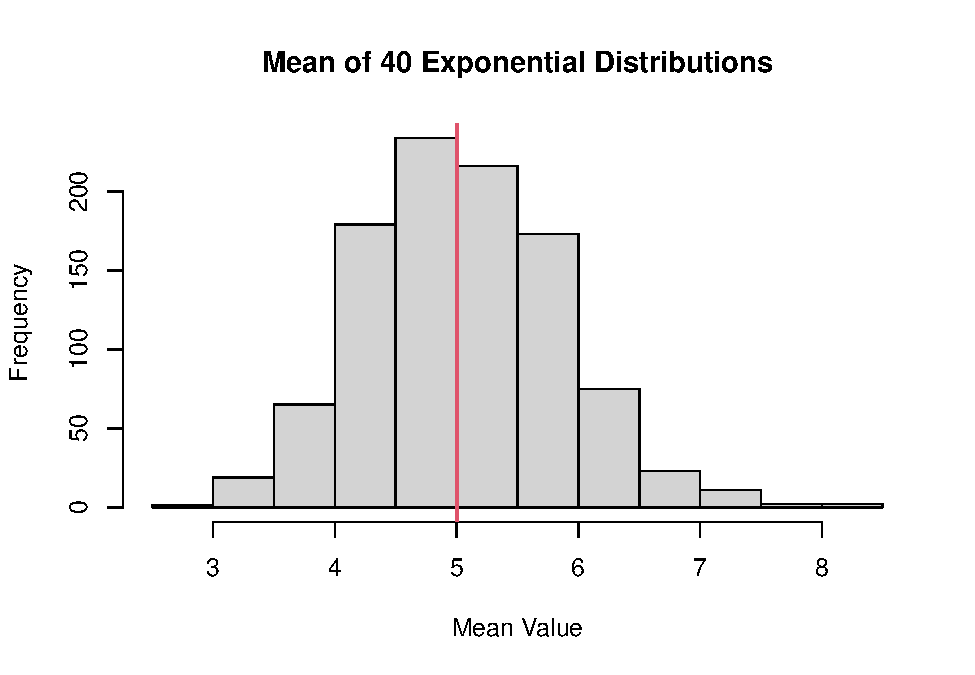
\includegraphics{Statistical-Inference-Project_files/figure-latex/unnamed-chunk-3-1.pdf}

In the plot above, we see a histogram of the 1000 means of the 40
exponential distributions. The theoretical mean is displayed as a
vertical red line. We can see that the most common mean value of 40
exponentials is approximately 5.

\hypertarget{sample-variance-versus-theoretical-variance}{%
\subsection{Sample Variance versus Theoretical
Variance}\label{sample-variance-versus-theoretical-variance}}

For the exponential distributions with a rate = lambda = 0.2 the
theoretical standard deviation is 1/lambda. The variance is equivalent
to the square of the standard deviation. Thus the theoretical variance
is equal to 25 = 5\^{}2.

\begin{Shaded}
\begin{Highlighting}[]
\NormalTok{sd\_theor\textless{}{-}}\DecValTok{1}\OperatorTok{/}\NormalTok{lambda}
\NormalTok{var\_sample\textless{}{-}}\KeywordTok{mean}\NormalTok{(vrs)}
\NormalTok{var\_theor\textless{}{-}sd\_theor}\OperatorTok{\^{}}\DecValTok{2}
\NormalTok{var\_sample}
\end{Highlighting}
\end{Shaded}

\begin{verbatim}
## [1] 25.02852
\end{verbatim}

\begin{Shaded}
\begin{Highlighting}[]
\NormalTok{var\_theor}
\end{Highlighting}
\end{Shaded}

\begin{verbatim}
## [1] 25
\end{verbatim}

We can see that the sample variance is in close agreement to the
theoretical variance of 25.

\begin{Shaded}
\begin{Highlighting}[]
\KeywordTok{hist}\NormalTok{(vrs,}\DataTypeTok{main=}\StringTok{"Variance of 40 Exponential Distributions"}\NormalTok{,}\DataTypeTok{xlab=}\StringTok{"Value"}\NormalTok{)}
\KeywordTok{abline}\NormalTok{(}\DataTypeTok{v=}\NormalTok{var\_theor,}\DataTypeTok{col=}\DecValTok{2}\NormalTok{,}\DataTypeTok{lwd=}\DecValTok{2}\NormalTok{)}
\end{Highlighting}
\end{Shaded}

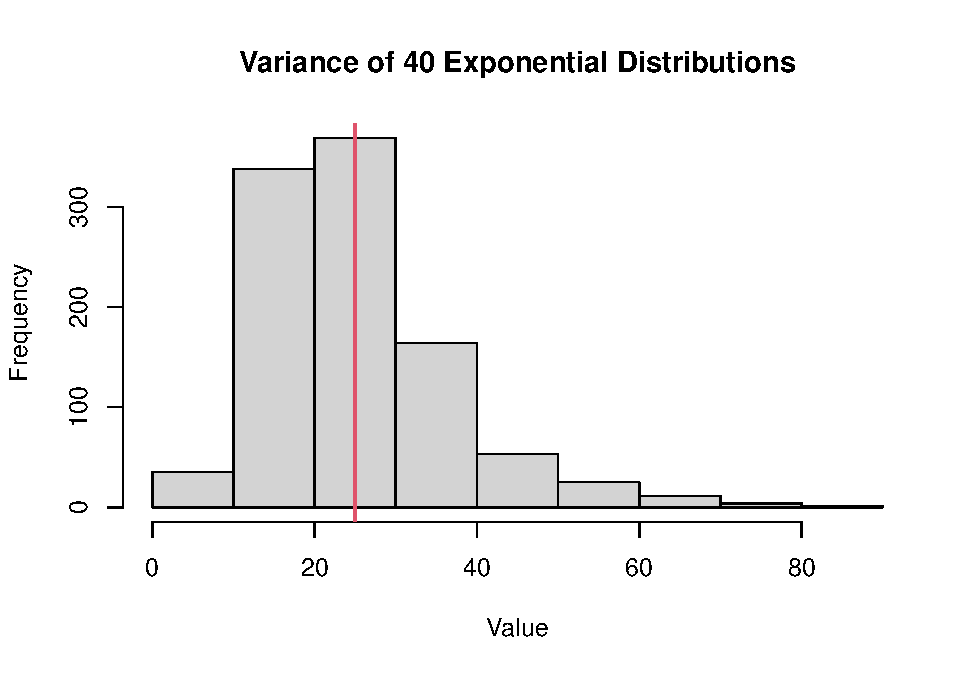
\includegraphics{Statistical-Inference-Project_files/figure-latex/unnamed-chunk-5-1.pdf}

In the plot above, we see a histogram of the 1000 variances of the 40
exponential distributions. The theoretical variance is displayed as a
vertical red line. We can see that the most common variance value of 40
exponentials is approximately 25.

\hypertarget{distribution}{%
\subsection{Distribution}\label{distribution}}

Below is the density histogram of the 1000 means of 40 exponentials.
Overlayed in red is a normal distribution curve.

\begin{Shaded}
\begin{Highlighting}[]
\KeywordTok{hist}\NormalTok{(mns,}\DataTypeTok{freq =} \OtherTok{FALSE}\NormalTok{,}\DataTypeTok{xlim=}\KeywordTok{c}\NormalTok{(}\DecValTok{0}\NormalTok{,}\DecValTok{10}\NormalTok{),}\DataTypeTok{main=}\StringTok{"Mean of 40 Exponential Distributions"}\NormalTok{,}\DataTypeTok{xlab=}\StringTok{"Mean Value"}\NormalTok{)}
\KeywordTok{curve}\NormalTok{(}\KeywordTok{dnorm}\NormalTok{(x,}\DataTypeTok{mean=}\NormalTok{mean\_theor,}\DataTypeTok{sd=}\DecValTok{1}\NormalTok{),}\DataTypeTok{add=}\OtherTok{TRUE}\NormalTok{,}\DataTypeTok{col=}\DecValTok{2}\NormalTok{,}\DataTypeTok{lwd=}\DecValTok{3}\NormalTok{)}
\end{Highlighting}
\end{Shaded}

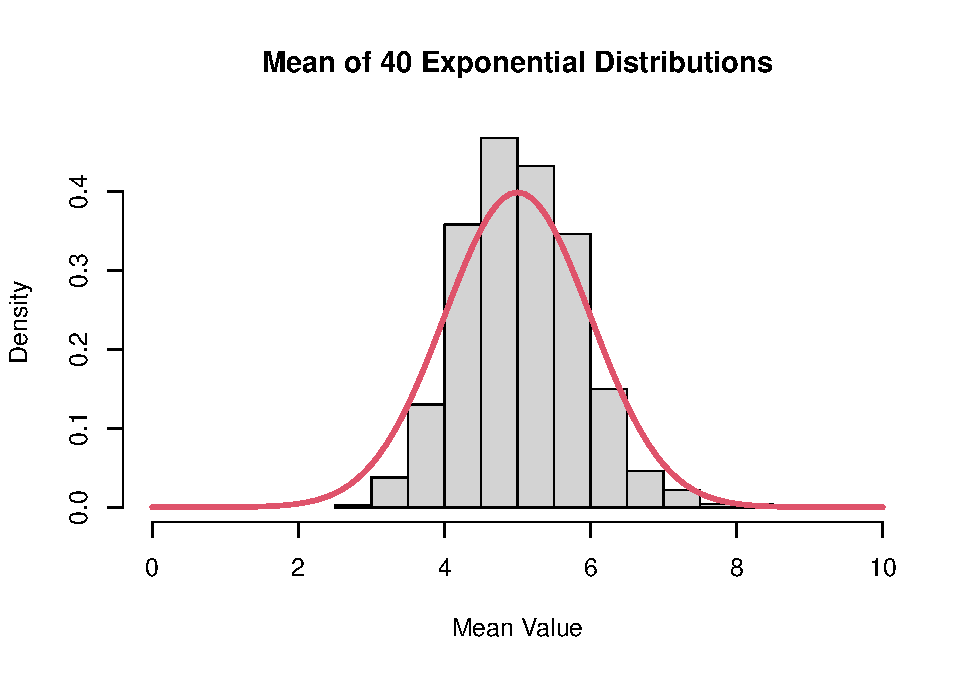
\includegraphics{Statistical-Inference-Project_files/figure-latex/unnamed-chunk-6-1.pdf}

We can see that the distribution of the means is approximately normal.
The histogram of the mean values as approximately the same shape as a
normal distribution curve centered at the theoretical mean.

\hypertarget{part-2-basic-inferential-data-analysis-exercise}{%
\section{Part 2: Basic Inferential Data Analysis
Exercise}\label{part-2-basic-inferential-data-analysis-exercise}}

We will use the Tooth Growth data set in R. It contains the tooth length
of guinea pigs who were given varying doses of Vitamin C through two
methods of administration (Orange Juice or Ascorbic Acid).

\begin{Shaded}
\begin{Highlighting}[]
\NormalTok{data\textless{}{-}ToothGrowth }\CommentTok{\#load and save data}
\KeywordTok{summary}\NormalTok{(data)}
\end{Highlighting}
\end{Shaded}

\begin{verbatim}
##       len        supp         dose      
##  Min.   : 4.20   OJ:30   Min.   :0.500  
##  1st Qu.:13.07   VC:30   1st Qu.:0.500  
##  Median :19.25           Median :1.000  
##  Mean   :18.81           Mean   :1.167  
##  3rd Qu.:25.27           3rd Qu.:2.000  
##  Max.   :33.90           Max.   :2.000
\end{verbatim}

\begin{Shaded}
\begin{Highlighting}[]
\KeywordTok{unique}\NormalTok{(data}\OperatorTok{$}\NormalTok{dose)}
\end{Highlighting}
\end{Shaded}

\begin{verbatim}
## [1] 0.5 1.0 2.0
\end{verbatim}

From the data summary we see that the tooth length varies from 4.2 to
33.9 with a median of 19.25 and a mean of 18.81. In addition we see that
there are 30 values each of tooth lengths for Vitamin C administered by
Orange Juice (OJ) and Ascorbic Acid (Vitamin C, VC). In addition we see
that the dose is either 0.5, 1.0, or 2.0 mg/day.

Below is code to isolate length by the Vitamin C delivery method and by
the dosage.

\begin{Shaded}
\begin{Highlighting}[]
\CommentTok{\# isolate length by Vitamin C delivery method}
\NormalTok{OJ\textless{}{-}data}\OperatorTok{$}\NormalTok{len[data}\OperatorTok{$}\NormalTok{supp}\OperatorTok{==}\StringTok{"OJ"}\NormalTok{] }\CommentTok{\#Orange Juice}
\NormalTok{VC\textless{}{-}data}\OperatorTok{$}\NormalTok{len[data}\OperatorTok{$}\NormalTok{supp}\OperatorTok{==}\StringTok{"VC"}\NormalTok{] }\CommentTok{\# Ascorbic Acid}

\CommentTok{\# isolate length by Vitamin C dosage [mg/day]}
\NormalTok{dose\_}\DecValTok{05}\NormalTok{\textless{}{-}data}\OperatorTok{$}\NormalTok{len[data}\OperatorTok{$}\NormalTok{dose}\OperatorTok{==}\FloatTok{0.5}\NormalTok{] }
\NormalTok{dose\_}\DecValTok{10}\NormalTok{\textless{}{-}data}\OperatorTok{$}\NormalTok{len[data}\OperatorTok{$}\NormalTok{dose}\OperatorTok{==}\FloatTok{1.0}\NormalTok{]}
\NormalTok{dose\_}\DecValTok{20}\NormalTok{\textless{}{-}data}\OperatorTok{$}\NormalTok{len[data}\OperatorTok{$}\NormalTok{dose}\OperatorTok{==}\FloatTok{2.0}\NormalTok{]}
\end{Highlighting}
\end{Shaded}

First, we will do hypothesis testing via a t-test to see if the toot
length differs based on the Vitamin C delivery method (supp).

\begin{Shaded}
\begin{Highlighting}[]
\KeywordTok{t.test}\NormalTok{(OJ,VC,}\DataTypeTok{paired=}\OtherTok{FALSE}\NormalTok{,}\DataTypeTok{alternative =} \StringTok{"two.sided"}\NormalTok{)}
\end{Highlighting}
\end{Shaded}

\begin{verbatim}
## 
##  Welch Two Sample t-test
## 
## data:  OJ and VC
## t = 1.9153, df = 55.309, p-value = 0.06063
## alternative hypothesis: true difference in means is not equal to 0
## 95 percent confidence interval:
##  -0.1710156  7.5710156
## sample estimates:
## mean of x mean of y 
##  20.66333  16.96333
\end{verbatim}

From the t-test we got a p-value of 0.06 which is greater than 0.05.
Hence, Tooth Growth was not significantly dependent on the delivery
method of Vitamin C.

There are three different doses. Since we did not cover ANOVAs in the
class I will do 3 t-tests and perform a p-value correction to see if
there is a significant difference. The threshold for significance is
equivalent to alpha = 0.05/3 = 0.0167.

First we will do a comparison of a dose of 0.5 mg/day compared to 2.0
mg/day.

\begin{Shaded}
\begin{Highlighting}[]
\KeywordTok{t.test}\NormalTok{(dose\_}\DecValTok{05}\NormalTok{,dose\_}\DecValTok{20}\NormalTok{,}\DataTypeTok{paired=}\OtherTok{FALSE}\NormalTok{,}\DataTypeTok{alternative =} \StringTok{"two.sided"}\NormalTok{)}
\end{Highlighting}
\end{Shaded}

\begin{verbatim}
## 
##  Welch Two Sample t-test
## 
## data:  dose_05 and dose_20
## t = -11.799, df = 36.883, p-value = 4.398e-14
## alternative hypothesis: true difference in means is not equal to 0
## 95 percent confidence interval:
##  -18.15617 -12.83383
## sample estimates:
## mean of x mean of y 
##    10.605    26.100
\end{verbatim}

We can see that tooth length is significantly dependent on the dosage of
Vitamin C of 0.5 compared to 2.0 mg/day.

Next, we will compare a dose of 0.5 mg/day compared to 1.0 mg/day.

\begin{Shaded}
\begin{Highlighting}[]
\KeywordTok{t.test}\NormalTok{(dose\_}\DecValTok{05}\NormalTok{,dose\_}\DecValTok{10}\NormalTok{,}\DataTypeTok{paired=}\OtherTok{FALSE}\NormalTok{,}\DataTypeTok{alternative =} \StringTok{"two.sided"}\NormalTok{)}
\end{Highlighting}
\end{Shaded}

\begin{verbatim}
## 
##  Welch Two Sample t-test
## 
## data:  dose_05 and dose_10
## t = -6.4766, df = 37.986, p-value = 1.268e-07
## alternative hypothesis: true difference in means is not equal to 0
## 95 percent confidence interval:
##  -11.983781  -6.276219
## sample estimates:
## mean of x mean of y 
##    10.605    19.735
\end{verbatim}

Again, we see that the tooth length for a 0.5 mg/day dose is
significantly different from that of a 1.0 mg/day dose.

Lastly, we will compare a dose of 1.0 mg/day compared to 2.0 mg/day.

\begin{Shaded}
\begin{Highlighting}[]
\KeywordTok{t.test}\NormalTok{(dose\_}\DecValTok{10}\NormalTok{,dose\_}\DecValTok{20}\NormalTok{,}\DataTypeTok{paired=}\OtherTok{FALSE}\NormalTok{,}\DataTypeTok{alternative =} \StringTok{"two.sided"}\NormalTok{)}
\end{Highlighting}
\end{Shaded}

\begin{verbatim}
## 
##  Welch Two Sample t-test
## 
## data:  dose_10 and dose_20
## t = -4.9005, df = 37.101, p-value = 1.906e-05
## alternative hypothesis: true difference in means is not equal to 0
## 95 percent confidence interval:
##  -8.996481 -3.733519
## sample estimates:
## mean of x mean of y 
##    19.735    26.100
\end{verbatim}

Once again, we see that the tooth length was significantly different for
Vitamin C doses of 1.0 compared to 2.0 mg/day.

Especially since we saw a significant difference between all comparisons
of 0.5, 1.0, and 2.0 mg/day with the adjusted p-value threshold we can
come to the conclusion that tooth length is significantly dependent on
the dosage of Vitamin C.

\end{document}
